\documentclass[conference]{IEEEtran}
% QONTOS Research Paper Series — Shared LaTeX Preamble
% Use with: % QONTOS Research Paper Series — Shared LaTeX Preamble
% Use with: % QONTOS Research Paper Series — Shared LaTeX Preamble
% Use with: \input{qontos-preamble}

\usepackage{cite}
\usepackage{amsmath,amssymb,amsfonts}
\usepackage{graphicx}
\usepackage{textcomp}
\usepackage{xcolor}
\usepackage{hyperref}
\usepackage{booktabs}
\usepackage{multirow}
\usepackage{array}
\usepackage{tabularx}
\usepackage{float}
\usepackage{listings}
\usepackage{url}
\usepackage{enumitem}

% Listing style
\lstset{
  basicstyle=\ttfamily\footnotesize,
  breaklines=true,
  frame=single,
  backgroundcolor=\color{gray!10},
}

% Custom column type
\newcolumntype{L}[1]{>{\raggedright\arraybackslash}p{#1}}

% QONTOS colors
\definecolor{qontosnavy}{HTML}{0A1628}
\definecolor{qontosblue}{HTML}{1E88E5}
\definecolor{qontosteal}{HTML}{00BCD4}

% Hyperref setup
\hypersetup{
  colorlinks=true,
  linkcolor=qontosblue,
  citecolor=qontosblue,
  urlcolor=qontosteal,
}

% Author block
\newcommand{\qontosauthor}{%
\IEEEauthorblockN{QONTOS Research Wing}
\IEEEauthorblockA{
Zhyra Quantum Research Institute (ZQRI)\\
Advanced Quantum Systems Division\\
Abu Dhabi, UAE\\
\texttt{research@zhyra.xyz}}
}


\usepackage{cite}
\usepackage{amsmath,amssymb,amsfonts}
\usepackage{graphicx}
\usepackage{textcomp}
\usepackage{xcolor}
\usepackage{hyperref}
\usepackage{booktabs}
\usepackage{multirow}
\usepackage{array}
\usepackage{tabularx}
\usepackage{float}
\usepackage{listings}
\usepackage{url}
\usepackage{enumitem}

% Listing style
\lstset{
  basicstyle=\ttfamily\footnotesize,
  breaklines=true,
  frame=single,
  backgroundcolor=\color{gray!10},
}

% Custom column type
\newcolumntype{L}[1]{>{\raggedright\arraybackslash}p{#1}}

% QONTOS colors
\definecolor{qontosnavy}{HTML}{0A1628}
\definecolor{qontosblue}{HTML}{1E88E5}
\definecolor{qontosteal}{HTML}{00BCD4}

% Hyperref setup
\hypersetup{
  colorlinks=true,
  linkcolor=qontosblue,
  citecolor=qontosblue,
  urlcolor=qontosteal,
}

% Author block
\newcommand{\qontosauthor}{%
\IEEEauthorblockN{QONTOS Research Wing}
\IEEEauthorblockA{
Zhyra Quantum Research Institute (ZQRI)\\
Advanced Quantum Systems Division\\
Abu Dhabi, UAE\\
\texttt{research@zhyra.xyz}}
}


\usepackage{cite}
\usepackage{amsmath,amssymb,amsfonts}
\usepackage{graphicx}
\usepackage{textcomp}
\usepackage{xcolor}
\usepackage{hyperref}
\usepackage{booktabs}
\usepackage{multirow}
\usepackage{array}
\usepackage{tabularx}
\usepackage{float}
\usepackage{listings}
\usepackage{url}
\usepackage{enumitem}

% Listing style
\lstset{
  basicstyle=\ttfamily\footnotesize,
  breaklines=true,
  frame=single,
  backgroundcolor=\color{gray!10},
}

% Custom column type
\newcolumntype{L}[1]{>{\raggedright\arraybackslash}p{#1}}

% QONTOS colors
\definecolor{qontosnavy}{HTML}{0A1628}
\definecolor{qontosblue}{HTML}{1E88E5}
\definecolor{qontosteal}{HTML}{00BCD4}

% Hyperref setup
\hypersetup{
  colorlinks=true,
  linkcolor=qontosblue,
  citecolor=qontosblue,
  urlcolor=qontosteal,
}

% Author block
\newcommand{\qontosauthor}{%
\IEEEauthorblockN{QONTOS Research Wing}
\IEEEauthorblockA{
Zhyra Quantum Research Institute (ZQRI)\\
Advanced Quantum Systems Division\\
Abu Dhabi, UAE\\
\texttt{research@zhyra.xyz}}
}


\begin{document}

\title{Tantalum-on-Silicon Superconducting Qubits: Materials and Device Feasibility for the QONTOS Hybrid Superconducting-Photonic Modular Architecture}
\author{\qontosauthor}
\maketitle

\begin{abstract}
This paper presents a materials and device feasibility analysis for the tantalum-on-silicon superconducting qubit platform as the candidate device layer for the QONTOS hybrid superconducting-photonic modular architecture. We evaluate coherence requirements, gate fidelity targets, fabrication yield constraints, chiplet packaging risks, control-line scaling limits, and calibration cadence demands across three architecture scenarios (base, aggressive, stretch). We analyze the relationship between coherence time and achievable logical depth, showing that $T_1$ approaching 1.7~ms with 25~ns gate times yields approximately 80,000 raw gate slots and that quantum error correction overhead reduces effective logical depth by one to two additional orders of magnitude. Literature-reported coherence advances~\cite{place2021, wang2022, bland2025} provide a credible starting point, but converting isolated device metrics into module-scale performance requires solving packaging, yield, calibration, and thermal integration problems that remain largely open. This paper maps those gaps honestly and defines the validation gates that must be cleared before stretch-scenario claims become defensible.

\textbf{Claim status:} Literature-informed device feasibility analysis with aggressive and stretch targets. This is a materials and device feasibility paper, not a performance demonstration.
\end{abstract}

\begin{IEEEkeywords}
superconducting qubits, transmon, tantalum, coherence, two-level systems, chiplet fabrication, device feasibility, quantum error correction overhead, hybrid superconducting-photonic architecture, photonic interconnects
\end{IEEEkeywords}

%% ----------------------------------------------------------------
\section{Introduction}

\subsection{Scope and Purpose}

The QONTOS hybrid superconducting-photonic modular architecture requires a superconducting qubit platform that simultaneously supports high coherence, high gate fidelity, scalable fabrication, modular packaging, and practical calibration and control. As the device layer for photonically-interconnected superconducting modules, the qubit platform must deliver performance that remains robust through integration into multi-chiplet cryogenic modules linked by photonic interconnects. Tantalum-on-silicon has emerged as an attractive candidate because recent literature reports demonstrate significant coherence improvements over earlier niobium- and aluminum-based material stacks~\cite{place2021, wang2022, bland2025}.

However, raw coherence values alone do not establish a viable path to fault-tolerant computation. This paper therefore focuses on what device-level performance would actually be needed for the QONTOS modular architecture to remain credible, and---equally important---which practical engineering barriers stand between reported single-device metrics and a functioning modular machine.

\textbf{[Claim: Scope]} This paper is a materials and device feasibility analysis. It does not report experimental results from QONTOS fabrication runs. All device metrics beyond published literature values are targets or assumptions, labeled as such throughout.

\subsection{Why Tantalum-on-Silicon}

The transmon qubit design~\cite{koch2007} has become the dominant superconducting qubit modality because of its relative insensitivity to charge noise and its compatibility with standard lithographic fabrication. The key limitation of transmon qubits has historically been energy relaxation ($T_1$), which is dominated by dielectric losses at material interfaces---particularly at the metal-substrate and metal-oxide boundaries where two-level system (TLS) defects reside~\cite{mueller2019}.

Tantalum offers specific materials advantages over niobium for superconducting qubit fabrication:

\begin{itemize}
\item Tantalum's native oxide (Ta$_2$O$_5$) appears to host fewer lossy TLS defects than niobium's native oxide (Nb$_2$O$_5$), as evidenced by the coherence improvements reported in~\cite{place2021, wang2022, bland2025}.
\item Epitaxial tantalum films can be grown on silicon substrates with well-controlled crystal orientation, reducing grain-boundary losses.
\item The tantalum-on-silicon material stack is compatible with standard semiconductor foundry processes, which is important for fabrication scaling.
\end{itemize}

\textbf{[Claim: Literature]} These advantages are supported by published literature but have been demonstrated primarily on isolated single-qubit or few-qubit devices. Performance at chiplet and module scale remains undemonstrated.

\subsection{Claim Status Summary}

\begin{table}[htbp]
\centering
\caption{Claim Status Summary.}
\label{tab:claims}
\begin{tabular}{lll}
\toprule
\textbf{Claim} & \textbf{Label} & \textbf{Status} \\
\midrule
$T_1 > 0.3$~ms in Ta transmons & LIT & Place et al.\ 2021~\cite{place2021} \\
$T_1 \approx 0.5$~ms demonstrated & LIT & Wang et al.\ 2022~\cite{wang2022} \\
$T_1 \sim 1.7$~ms on isolated devices & LIT & Bland et al.\ 2025~\cite{bland2025} \\
Stretch arch.\ assumes 2~ms $T_1$ & TARGET & Undemonstrated \\
99.999\% 2Q gate fidelity at scale & STRETCH & Undemonstrated \\
Chiplet yield for 10k-qubit modules & STRETCH & Undemonstrated \\
Fab scalable to million-qubit regime & STRETCH & Speculative \\
\bottomrule
\end{tabular}
\end{table}

%% ----------------------------------------------------------------
\section{Device Performance Requirements}

\subsection{Scenario-Based Targets}

The QONTOS architecture defines three device performance scenarios. Each represents a different level of ambition and a different burden of proof.

\begin{table}[htbp]
\centering
\caption{Scenario-Based Device Targets.}
\label{tab:device_targets}
\begin{tabular}{lrrrl}
\toprule
\textbf{Metric} & \textbf{Base} & \textbf{Aggr.} & \textbf{Stretch} & \textbf{Label} \\
\midrule
$T_1$ & 300~$\mu$s & 1~ms & 2~ms & Target \\
$T_2$ & 300~$\mu$s & 1~ms & 1.5--2~ms & Target \\
1Q gate fidelity & 99.9\% & 99.99\% & 99.999\% & Target \\
2Q gate fidelity & 99.9\% & 99.99\% & 99.999\% & Target \\
2Q gate time & 50~ns & 35~ns & 25~ns & Target \\
Readout fidelity & 99.5\% & 99.9\% & 99.99\% & Target \\
Readout time & 500~ns & 300~ns & 200~ns & Target \\
\bottomrule
\end{tabular}
\end{table}

\textbf{[Claim: Target]} The base scenario is consistent with current state-of-the-art demonstrations on small devices. The aggressive scenario requires meaningful advances in gate calibration and packaging. The stretch scenario has not been demonstrated on any platform at multi-qubit scale.

\subsection{Literature Baseline}

\begin{figure}[htbp]
\centering
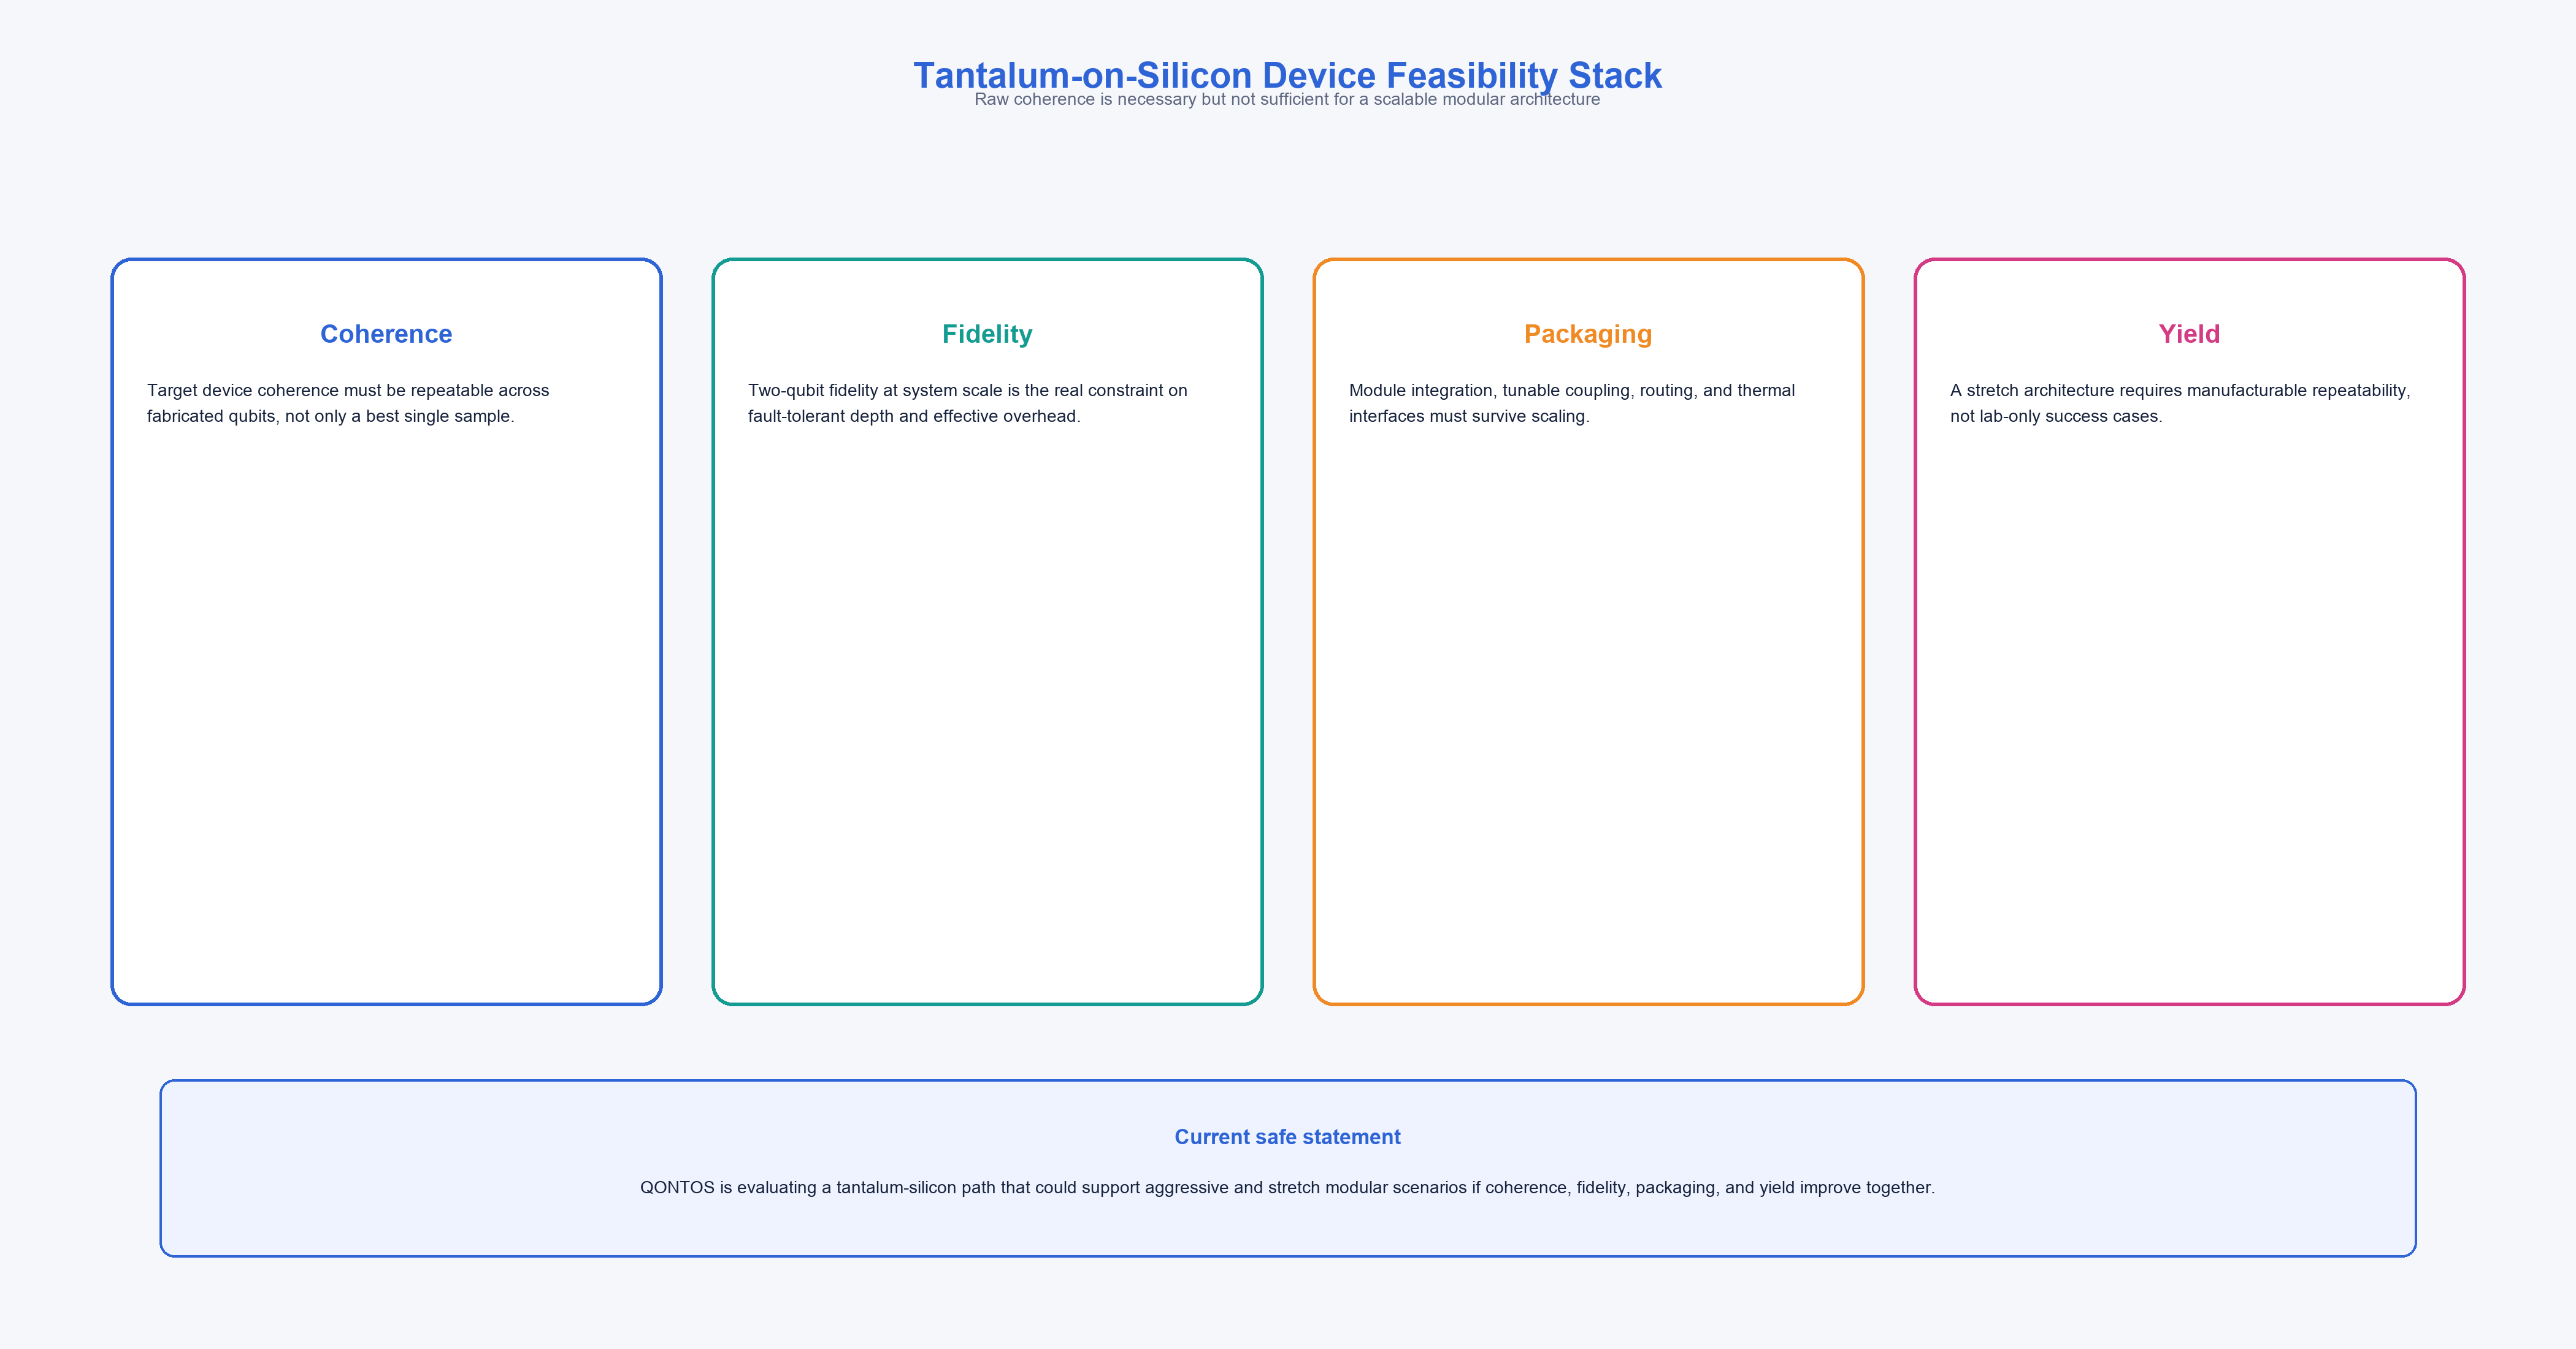
\includegraphics[width=\columnwidth]{../../figures/02_qubit_physics.png}
\caption{Coherence Progress in Tantalum Transmons.}
\label{fig:coherence_progress}
\end{figure}

The current literature establishes the following trajectory for tantalum transmon coherence:

\begin{table}[htbp]
\centering
\caption{Literature Coherence Baseline.}
\label{tab:lit_baseline}
\begin{tabular}{llrll}
\toprule
\textbf{Reference} & \textbf{Year} & \textbf{$T_1$} & \textbf{Platform} & \textbf{Scale} \\
\midrule
Place et al.~\cite{place2021} & 2021 & 0.3~ms & Ta on sapphire & Single qubit \\
Wang et al.~\cite{wang2022} & 2022 & 0.5~ms & Ta transmon & Single qubit \\
Bland et al.~\cite{bland2025} & 2025 & 1.68~ms & Ta on silicon & Single qubit \\
\bottomrule
\end{tabular}
\end{table}

\textbf{[Claim: Literature]} These results establish that millisecond-class $T_1$ is physically achievable in tantalum transmon devices. They do not establish that this coherence survives integration into multi-qubit chiplets, packaging assemblies, or operating modules with active control electronics. The gap between isolated-device coherence and system-level coherence is historically large in superconducting qubit platforms~\cite{kjaergaard2020}.

\subsection{The TLS Loss Budget}

Coherence in superconducting transmons is limited by energy relaxation into TLS defects at material interfaces~\cite{mueller2019}. The total loss rate can be decomposed as:

\begin{equation}
\frac{1}{T_{1,\text{total}}} = \frac{1}{T_{1,\text{bulk}}} + \frac{1}{T_{1,\text{surface}}} + \frac{1}{T_{1,\text{interface}}} + \frac{1}{T_{1,\text{radiation}}} + \frac{1}{T_{1,\text{other}}}
\end{equation}

For tantalum-on-silicon devices, the dominant terms are:

\begin{itemize}
\item \textbf{Surface and interface losses:} TLS defects at the tantalum-oxide and substrate interfaces. Tantalum's advantage lies primarily in reducing these terms.
\item \textbf{Radiation losses:} Coupling to spurious electromagnetic modes in the package or chip environment. These losses are independent of materials quality and become dominant once surface losses are suppressed.
\item \textbf{Bulk losses:} Typically negligible for high-purity tantalum on high-resistivity silicon.
\end{itemize}

\textbf{[Claim: Analysis]} Reaching the stretch $T_1$ target of 2~ms at scale requires suppressing all loss channels simultaneously. Materials improvement alone (reducing surface TLS) is necessary but not sufficient. Packaging-induced radiation losses and thermally activated TLS contributions under operating conditions must also be controlled.

%% ----------------------------------------------------------------
\section{Coherence, Gate Time, and Logical Depth}

\begin{figure}[htbp]
\centering
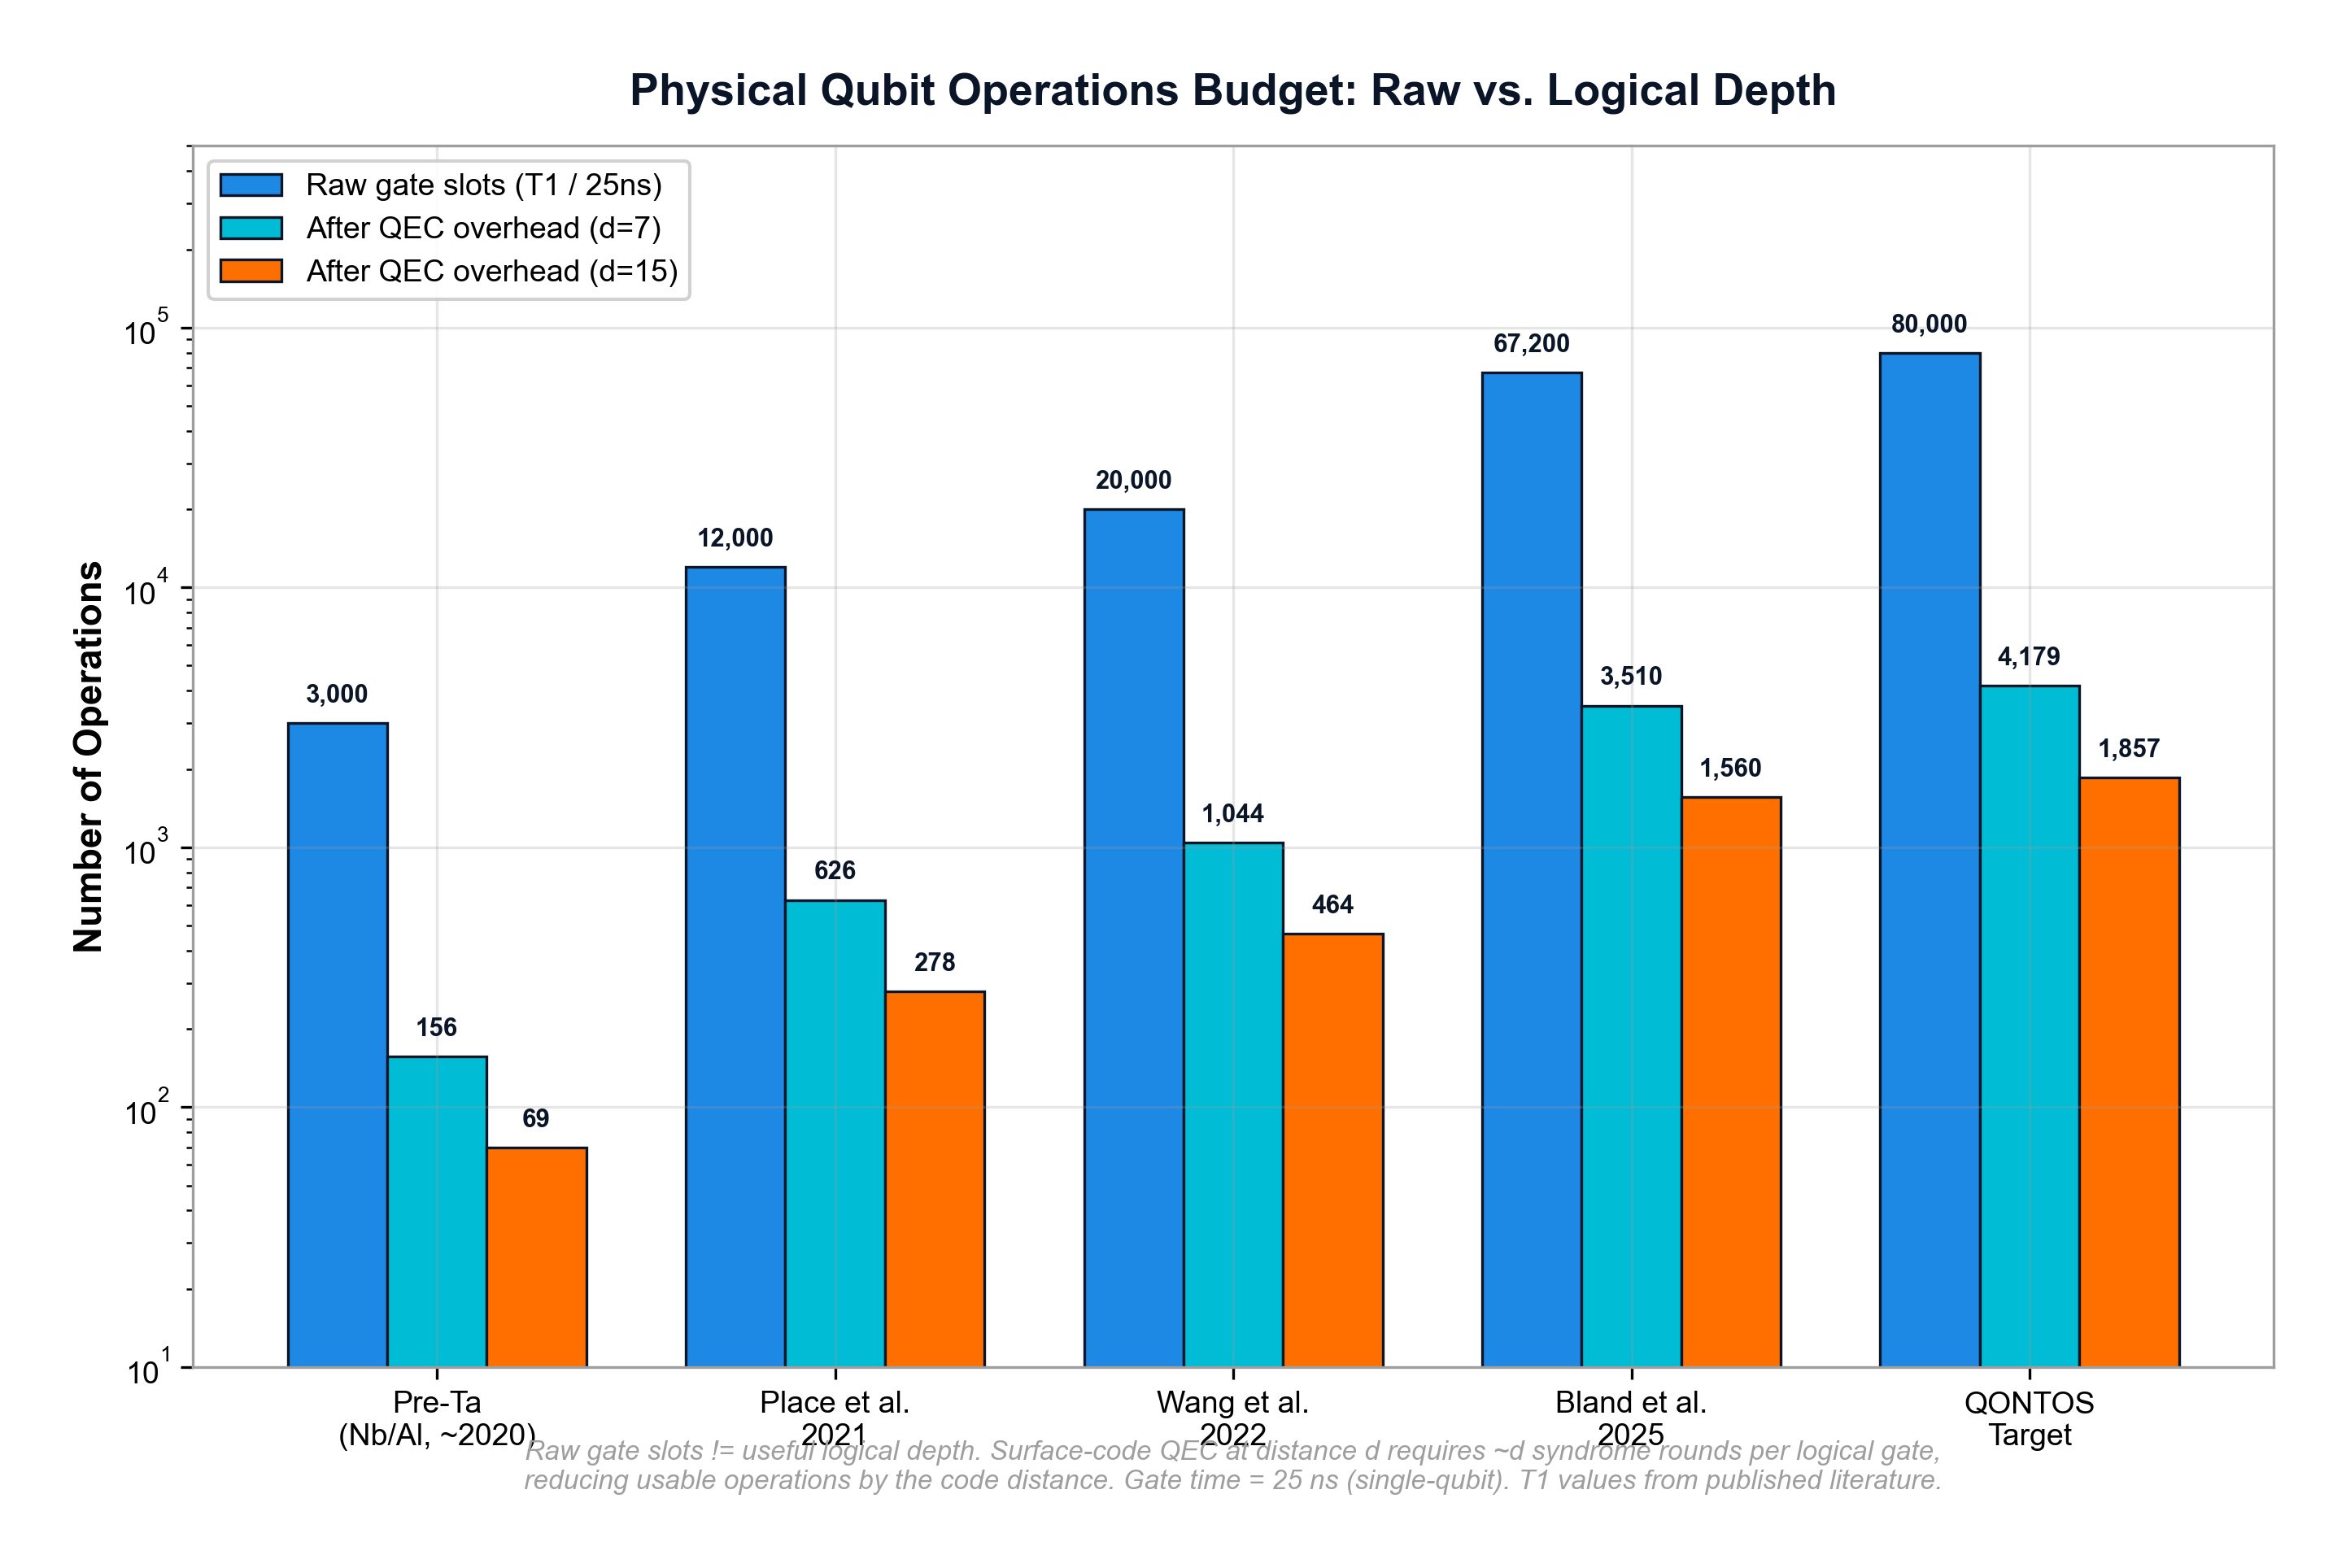
\includegraphics[width=\columnwidth]{../../figures/02_materials_comparison.png}
\caption{Operations Budget Analysis.}
\label{fig:ops_budget}
\end{figure}

\subsection{Operations-Count Analysis}

A common approach in quantum computing roadmap documents is to equate raw coherence time with computational capacity by dividing $T_1$ by gate time and presenting the result as the number of available operations. This calculation requires careful analysis.

\textbf{The raw arithmetic:}

\begin{equation}
\text{Raw physical gate slots} = T_1 / t_{\text{gate}}
\end{equation}

For stretch targets: $T_1 = 2$~ms, 2Q gate time $= 25$~ns:
\begin{equation}
\text{Raw gate slots} = \frac{2{,}000{,}000~\text{ns}}{25~\text{ns}} = 80{,}000
\end{equation}

\textbf{[Claim: Analysis]} The result is 80,000 raw physical gate slots. It is important to distinguish this figure from the effective logical depth available after accounting for error correction overhead, as detailed below.

\subsection{From Raw Gate Slots to Effective Logical Depth}

Even 80,000 raw gate slots substantially overstates the useful computational depth available for a fault-tolerant algorithm. The following overhead factors must be applied:

\begin{table}[htbp]
\centering
\caption{From Raw Gate Slots to Logical Depth.}
\label{tab:depth_reduction}
\begin{tabular}{lrr}
\toprule
\textbf{Overhead source} & \textbf{Reduction} & \textbf{Remaining} \\
\midrule
Raw physical ($T_1/t_{\text{gate}}$) & --- & 80,000 \\
QEC syndrome (${\sim}1$~$\mu$s each) & $\times$50--100 & 800--1,600 \\
Decoder latency \& feedback & 1.2--2$\times$ & 400--1,300 \\
Idling errors during syndrome & Variable & Further reduced \\
State prep \& measurement & Fixed/comp. & Further reduced \\
Calibration drift & Variable & Further reduced \\
\bottomrule
\end{tabular}
\end{table}

\textbf{[Claim: Analysis]} Under realistic assumptions for surface-code QEC with code distance $d = 15$--$21$, the effective logical circuit depth available from a 2~ms $T_1$ device with 25~ns gates is on the order of several hundred to low thousands of logical operations. This depth is meaningful and potentially sufficient for certain classes of algorithms, and it is important to characterize it accurately for architecture planning purposes.

The QEC refresh cycle is the critical bottleneck. In the surface code, syndrome extraction requires measuring all stabilizer operators, which takes approximately $d$ rounds of measurements at roughly 1~$\mu$s per round for code distance $d$~\cite{sheldon2016}. During this time, the physical qubits are accumulating errors. Every logical gate thus consumes on the order of $d$ to several-$d$ microseconds of physical coherence time.

For the stretch scenario with $d = 17$:

\begin{align}
&\text{Syndrome extraction time per QEC round:} \sim 1~\mu\text{s} \nonumber \\
&\text{Rounds per logical gate:} \sim 17 \nonumber \\
&\text{Physical time per logical gate:} \sim 17~\mu\text{s} \nonumber \\
&\text{Available logical gates from } T_1 = 2~\text{ms:} \nonumber \\
&\quad \sim 2000~\mu\text{s} / 17~\mu\text{s} \approx 120 \text{ logical gates} \nonumber
\end{align}

\textbf{[Claim: Analysis]} This is a conservative lower bound; pipelining and code optimizations can improve this by factors of 2--5$\times$ depending on the algorithm structure. But the fundamental point stands: the useful logical depth from millisecond-class coherence is measured in hundreds to low thousands, not in millions or billions.

\subsection{Why This Still Matters}

Despite the dramatic reduction from raw gate slots to effective logical depth, millisecond-class coherence is genuinely valuable for three reasons:

\begin{enumerate}
\item \textbf{Reduced code distance:} Higher $T_1$ means lower physical error rates, which reduces the code distance required for a given logical error rate. Reducing $d$ from 21 to 15 approximately halves the physical qubit overhead per logical qubit.
\item \textbf{Wider error budget:} More coherence time provides margin for other error sources (leakage, cross-talk, calibration drift) without exceeding the QEC threshold.
\item \textbf{Longer syndrome extraction windows:} More time per QEC cycle allows slower, more reliable measurement without coherence-induced failures.
\end{enumerate}

\textbf{[Claim: Analysis]} The honest value proposition of 2~ms $T_1$ is not ``enormous computational depth'' but rather ``reduced overhead and wider engineering margins for fault tolerance.'' This framing is less dramatic but more defensible.

\subsection{Workload-Oriented Device Requirements}

\begin{table}[htbp]
\centering
\caption{Workload-Oriented Device Requirements.}
\label{tab:workload_reqs}
\begin{tabular}{rrp{3cm}}
\toprule
\textbf{Workload class} & \textbf{Log.\ depth} & \textbf{Device regime} \\
\midrule
Early logical-qubit demos & 10--100 & Base to aggressive \\
Quantum advantage benchmarks & 100--1,000 & Aggressive \\
Modular FT demonstrations & 1k--10k & Aggressive to stretch \\
FeMoco-class flagship & 10,000+ & Stretch + interconnect + decoder \\
\bottomrule
\end{tabular}
\end{table}

\textbf{[Claim: Target]} The FeMoco workload class requires stretch device performance AND significant advances in QEC, decoding, and modular interconnects. No single improvement in device coherence is sufficient.

%% ----------------------------------------------------------------
\section{Device Architecture and Control}

\subsection{Transmon-Coupler Topology}

The QONTOS architecture assumes a tunable-coupler transmon topology for two-qubit interactions. The tunable coupler mediates interactions between fixed-frequency transmon qubits, enabling fast controlled-Z (CZ) or cross-resonance (CR) gates~\cite{sheldon2016} while suppressing residual ZZ coupling during idle periods.

\begin{table}[htbp]
\centering
\caption{Tunable-Coupler Parameters.}
\label{tab:coupler}
\begin{tabular}{lrrl}
\toprule
\textbf{Parameter} & \textbf{Aggr.} & \textbf{Stretch} & \textbf{Label} \\
\midrule
Coupling range & $\pm 50$~MHz & $\pm 50$~MHz & Target \\
CZ gate fidelity & 99.99\% & 99.999\% & Target \\
CZ gate time & 35~ns & 25~ns & Target \\
ZZ suppression (idle) & $< 1$~kHz & $< 0.1$~kHz & Target \\
Freq.\ targeting accuracy & $\pm 20$~MHz & $\pm 10$~MHz & Target \\
\bottomrule
\end{tabular}
\end{table}

\subsection{Frequency Crowding and Collision Avoidance}

As qubit count per chiplet increases, frequency allocation becomes a combinatorial constraint. Each transmon must operate at a frequency that avoids collisions with neighboring qubits' fundamental and higher-level transitions. The standard transmon has an anharmonicity of approximately $-200$ to $-300$~MHz~\cite{koch2007}, creating exclusion zones around each qubit frequency.

\textbf{[Claim: Analysis]} For a 2,000-qubit chiplet with nearest-neighbor connectivity, frequency allocation requires careful layout optimization. The probability of at least one frequency collision scales unfavorably with qubit count unless frequency targeting accuracy improves to better than $\pm 15$~MHz. Laser-annealing-based frequency trimming may mitigate this, but adds process complexity.

\subsection{Packaging and Yield Risks}

This section addresses risks that are absent from most coherence-focused literature but are critical for the QONTOS modular architecture.

\subsubsection{Wafer-Level Yield Assumptions}

\textbf{[Claim: Target]} The stretch architecture assumes 2,000 functional qubits per chiplet. The yield implications are severe:

\begin{table}[htbp]
\centering
\caption{Yield Scenario Analysis.}
\label{tab:yield}
\begin{tabular}{rrrl}
\toprule
\textbf{Yield} & \textbf{Defective/2k} & \textbf{Pass rate} & \textbf{Label} \\
\midrule
99.9\% & 2 & ${\sim}13\%$ & Analysis \\
99.95\% & 1 & ${\sim}37\%$ & Analysis \\
99.99\% & 0.2 & ${\sim}82\%$ & Analysis \\
\bottomrule
\end{tabular}
\end{table}

These estimates assume independent, identically distributed defect probabilities---an optimistic assumption, since defects tend to cluster spatially on wafers.

\textbf{[Claim: Analysis]} At 99.9\% per-qubit yield, only about 1 in 8 chiplets would be defect-free. The architecture must either achieve 99.99\%+ qubit yield (unprecedented for superconducting qubit fabrication) or incorporate defect-tolerant design features such as spare qubits, reroutable couplers, or post-fabrication frequency trimming.

\subsubsection{Chiplet Packaging Limits}

The chiplet-to-module packaging step introduces several risk factors:

\begin{itemize}
\item \textbf{Bump-bond yield:} Each chiplet requires hundreds of superconducting bump bonds for inter-chiplet coupling and signal routing. Even 99.9\% bump-bond yield becomes problematic at 500+ bonds per chiplet.
\item \textbf{Thermal cycling degradation:} Repeated cool-down and warm-up cycles stress mechanical interfaces and can degrade bump-bond integrity over the module lifetime.
\item \textbf{Coherence degradation from packaging:} Published single-device $T_1$ values are measured in optimized test fixtures. Packaging into multi-chiplet modules introduces additional loss channels (spurious modes, radiation from wirebonds or bump bonds, substrate coupling) that typically reduce $T_1$ by 2--5$\times$~\cite{kjaergaard2020}.
\end{itemize}

\textbf{[Claim: Risk]} The gap between test-fixture coherence and packaged-module coherence is the single largest risk to the stretch architecture's device assumptions. A 2~ms test-fixture $T_1$ may yield only 0.4--1.0~ms in a packaged module, which changes the feasibility analysis substantially.

\subsubsection{Defect Tolerance Strategy}

For the stretch architecture to survive realistic yield, the following defect tolerance mechanisms should be evaluated:

\begin{enumerate}
\item \textbf{Spare qubit rows/columns:} Allocating 5--10\% additional qubits per chiplet as spares, with reroutable coupling.
\item \textbf{Post-fabrication screening:} Testing each chiplet at cryogenic temperatures before module assembly, discarding defective units.
\item \textbf{Frequency trimming:} Laser annealing or other post-fabrication tuning to correct frequency collisions without redesign.
\end{enumerate}

\textbf{[Claim: Target]} None of these mechanisms have been demonstrated at the 2,000-qubit chiplet scale. Each adds fabrication complexity and cost.

%% ----------------------------------------------------------------
\section{Fabrication and Packaging Strategy}

\subsection{Chiplet Architecture Assumptions}

The QONTOS stretch architecture assumes:

\begin{table}[htbp]
\centering
\caption{Chiplet Architecture Parameters.}
\label{tab:chiplet_arch}
\begin{tabular}{lrl}
\toprule
\textbf{Parameter} & \textbf{Value} & \textbf{Label} \\
\midrule
Physical qubits/chiplet & 2,000 & Target \\
Chiplets/module & 5 & Target \\
Physical qubits/module & 10,000 & Target \\
Inter-chiplet coupling channels & 50--100/edge & Target \\
Chiplet die size & ${\sim}20 \times 20$~mm & Target \\
\bottomrule
\end{tabular}
\end{table}

\textbf{[Claim: Target]} These are architecture constants derived from system-level modeling, not demonstrated manufacturing outputs. The largest demonstrated superconducting qubit chiplets as of 2025 contain on the order of 100--200 qubits.

\subsection{Control and Calibration Implications}

\subsubsection{Control Line Scaling}

Each transmon qubit requires at minimum:

\begin{itemize}
\item 1 XY drive line (microwave, ${\sim}5$~GHz)
\item 1 flux bias line (DC or low-frequency, for tunable couplers)
\item 1 readout resonator coupling (shared multiplexed line, typically 4--8 qubits per line)
\end{itemize}

For a 2,000-qubit chiplet, the control line count is approximately:

\begin{align}
&\text{XY drive lines: } 2{,}000 \nonumber \\
&\text{Flux lines (couplers): } {\sim}1{,}000\text{--}2{,}000 \nonumber \\
&\text{Readout lines (mux): } {\sim}250\text{--}500 \nonumber \\
&\text{Total per chiplet: } {\sim}3{,}250\text{--}4{,}500 \nonumber
\end{align}

\textbf{[Claim: Analysis]} Routing 3,000+ control lines to a 20~mm $\times$ 20~mm chiplet at millikelvin temperatures is an unsolved packaging problem. Current cryogenic wiring technology~\cite{krinner2019} supports on the order of 200--400 coaxial lines per dilution refrigerator. Frequency-multiplexed and cryogenic-CMOS control approaches are under development but remain immature.

\subsubsection{Calibration Cadence and Drift}

Transmon qubits require periodic recalibration of qubit frequencies (drift due to TLS fluctuations), gate pulse parameters (amplitude, frequency, phase, DRAG corrections), readout discriminator thresholds, and coupler bias points.

\textbf{[Claim: Analysis]} Current calibration cadence for state-of-the-art devices is approximately every 1--4 hours for single-qubit gate parameters and every 15--60 minutes for two-qubit gate parameters. For a 2,000-qubit chiplet, sequential calibration of all gates would require:

\begin{align}
&2{,}000 \text{ 1Q gates} \times {\sim}30\text{~s each} = {\sim}17\text{~hours (sequential)} \nonumber \\
&{\sim}3{,}000 \text{ 2Q gates} \times {\sim}60\text{~s each} = {\sim}50\text{~hours (sequential)} \nonumber
\end{align}

This is obviously infeasible sequentially. Parallel calibration protocols are required, but these introduce cross-talk artifacts that must themselves be characterized and corrected~\cite{sheldon2016}.

\textbf{[Claim: Risk]} Calibration automation at the 2,000-qubit scale is an unsolved engineering problem. The stretch architecture implicitly assumes that calibration can be fully automated and parallelized with sub-hour turnaround times. This assumption should be treated as a first-order risk.

\subsubsection{Control Electronics Scaling}

The control electronics stack for a 10,000-qubit module (5 chiplets) requires:

\begin{table}[htbp]
\centering
\caption{Control Electronics Requirements per Module.}
\label{tab:ctrl_electronics}
\begin{tabular}{lrp{2.5cm}}
\toprule
\textbf{Component} & \textbf{Count} & \textbf{State of the art} \\
\midrule
MW signal generators & ${\sim}10{,}000$ ch. & ${\sim}100$--200/rack \\
Arb.\ waveform gen. & ${\sim}10{,}000$ ch. & ${\sim}100$--200/rack \\
DC bias sources & 5k--10k & ${\sim}500$/rack \\
Digitizers (readout) & 1.25k--2.5k & ${\sim}100$/rack \\
\bottomrule
\end{tabular}
\end{table}

\textbf{[Claim: Analysis]} The electronics footprint for a single stretch module would occupy approximately 50--100 equipment racks with current commercial hardware. Room-temperature-to-cryostat wiring would require hundreds of coaxial cables per module~\cite{krinner2019}. Cryogenic control integration (CMOS or SFQ logic at the 4K or mK stage) could reduce this dramatically but remains at the research prototype stage.

\subsection{Fabrication Partner Strategy}

\textbf{[Claim: Target]} QONTOS is exploring a multi-partner fabrication strategy to reduce supply-chain concentration and improve scale flexibility. Specific partner details are not disclosed in this feasibility paper.

The relevant fabrication questions are:

\begin{table}[htbp]
\centering
\caption{Key Fabrication Questions.}
\label{tab:fab_questions}
\begin{tabular}{lp{3cm}l}
\toprule
\textbf{Question} & \textbf{Why it matters} & \textbf{Label} \\
\midrule
Yield $> 99.95\%$/qubit? & Chiplet economics & Risk \\
Packaging preserves $> 80\%$ $T_1$? & Module coherence & Risk \\
Freq.\ targeting $\pm 10$~MHz? & Collision avoidance & Risk \\
Foundry Ta film quality? & Coherence depends on it & Risk \\
\bottomrule
\end{tabular}
\end{table}

%% ----------------------------------------------------------------
\section{Thermal and Integration Constraints}

\subsection{Module Thermal Envelope}

The millikelvin stage of a dilution refrigerator provides a limited cooling power budget, typically 10--25~$\mu$W at 20~mK for standard commercial units, scaling to ${\sim}25$~mW at the mixing chamber plate (which operates at ${\sim}20$--50~mK)~\cite{krinner2019}. The module thermal budget must account for:

\begin{table}[htbp]
\centering
\caption{Module Thermal Budget.}
\label{tab:thermal}
\begin{tabular}{lrl}
\toprule
\textbf{Heat source} & \textbf{Est.\ load/module} & \textbf{Label} \\
\midrule
Coaxial signal lines (passive) & ${\sim}20$~mW at MXC & Estimate \\
Optical fiber terminations & ${\sim}0.01$~mW & Estimate \\
DC bias lines & ${\sim}0.5$~mW & Estimate \\
Chip dissipation (gates + readout) & ${\sim}0.1$~mW & Estimate \\
\textbf{Total estimated load} & ${\sim}21$~mW & Estimate \\
\textbf{Available thermal budget} & ${\sim}25$~mW & Estimate \\
\bottomrule
\end{tabular}
\end{table}

\textbf{[Claim: Risk]} The thermal margin is approximately 4~mW, or about 19\% of the total budget. This provides minimal contingency for packaging heat leaks, wiring thermal anchoring imperfections, or control electronics heat dissipation if any cryogenic control is integrated at the mixing chamber stage. The thermal envelope is one of the hardest constraints on module scale.

\subsection{Validation Gates}

The materials and device feasibility claims in this paper require the following validation milestones before the stretch architecture can be considered credible:

\subsubsection{Gate V1: Packaged Coherence Validation}

\textbf{Requirement:} Demonstrate $T_1 > 1$~ms and $T_2 > 0.8$~ms in a multi-qubit device ($\geq 10$ qubits) after full chiplet packaging (bump bonds, interposer, enclosure).

\textbf{Rationale:} This validates that packaging does not destroy the coherence advantage of tantalum. Current literature reports are exclusively on isolated test devices.

\textbf{Status:} Not demonstrated. \textbf{[Claim: Gate]}

\subsubsection{Gate V2: Chiplet Yield Demonstration}

\textbf{Requirement:} Fabricate and test $\geq 10$ chiplets of $\geq 100$ qubits each with per-qubit yield exceeding 99.5\% and median $T_1$ exceeding 500~$\mu$s.

\textbf{Rationale:} This validates fabrication consistency and provides the first statistical basis for yield projections at the 2,000-qubit scale.

\textbf{Status:} Not demonstrated. \textbf{[Claim: Gate]}

\subsubsection{Gate V3: Calibration Automation at Scale}

\textbf{Requirement:} Demonstrate automated calibration of a $\geq 50$-qubit device with all single-qubit and two-qubit gates achieving target fidelity within 1 hour, with calibration remaining valid for $\geq 4$ hours.

\textbf{Rationale:} This validates that calibration can keep pace with device scale.

\textbf{Status:} Not demonstrated. \textbf{[Claim: Gate]}

\subsubsection{Gate V4: Thermal Budget Validation}

\textbf{Requirement:} Operate a multi-chiplet assembly ($\geq 2$ chiplets, $\geq 200$ qubits) within the thermal budget of a single dilution refrigerator mixing chamber stage, with base temperature remaining below 25~mK.

\textbf{Rationale:} This validates that module-scale integration is thermally feasible.

\textbf{Status:} Not demonstrated. \textbf{[Claim: Gate]}

\subsubsection{Gate V5: System-Level Coherence Under Load}

\textbf{Requirement:} Demonstrate that $T_1$ degradation under simultaneous operation of all qubits in a chiplet (gates + readout + idle) does not exceed 30\% relative to single-qubit isolated measurements.

\textbf{Rationale:} Crosstalk, heating, and control interference typically degrade coherence under realistic operating conditions. The architecture assumptions require bounded degradation.

\textbf{Status:} Not demonstrated. \textbf{[Claim: Gate]}

%% ----------------------------------------------------------------
\section{Device Roadmap by Scenario}

\subsection{Timeline Mapping}

\begin{table*}[htbp]
\centering
\caption{Device Roadmap by Phase and Scenario.}
\label{tab:roadmap}
\begin{tabular}{lp{3.5cm}p{3.5cm}p{4cm}}
\toprule
\textbf{Phase} & \textbf{Base} & \textbf{Aggressive} & \textbf{Stretch} \\
\midrule
2025--2026 & Lit.\ benchmarking; design studies; calibration tooling & Small-scale internal validation (5--20 qubits) & First evidence $T_1 > 1$~ms in packaged multi-qubit devices \\
2026--2027 & Device-package integration; yield char. & Module-scale targets (100+ qubits) & Gate V1 and V2 milestones attempted \\
2027--2028 & Robust modular HW with base-level specs & High-fidelity chiplet fleet (500+ qubits) & V3, V4, V5 milestones; 2k-qubit prototypes \\
2028--2029 & Production-quality base modules & Multi-module demos & Arch.-scale stretch envelope tested \\
2029--2030 & Strong device basis for modular products & Large-scale modular FT path & Full stretch assumptions validated or revised \\
\bottomrule
\end{tabular}
\end{table*}

\textbf{[Claim: Target]} This roadmap assumes sustained funding, successful partner engagement, and no fundamental materials or engineering barriers beyond those identified in this paper. Each transition between phases is contingent on clearing the relevant validation gates.

\subsection{Risk-Adjusted Expectations}

\begin{table}[htbp]
\centering
\caption{Risk-Adjusted Success Probabilities.}
\label{tab:risk_adjusted}
\begin{tabular}{lrp{3cm}}
\toprule
\textbf{Scenario} & \textbf{P(success by 2030)} & \textbf{Primary risk} \\
\midrule
Base & $> 70\%$ & Execution and funding \\
Aggressive & 30--50\% & Packaging coherence loss; calibration \\
Stretch & 10--25\% & Yield, packaging, control, calibration---all simultaneously \\
\bottomrule
\end{tabular}
\end{table}

\textbf{[Claim: Analysis]} The stretch scenario requires simultaneous success across multiple independent engineering dimensions. The probability of achieving all stretch targets on schedule is the product of individual success probabilities, which compounds unfavorably. This does not mean the stretch scenario is impossible, but it should be planned as a best-case outcome, not an expected one.

%% ----------------------------------------------------------------
\section{Open Questions and Research Priorities}

\subsection{Materials Science}

\begin{enumerate}
\item What is the intrinsic TLS loss limit of the tantalum-silicon interface under optimal growth conditions?
\item Can tantalum film quality be maintained in foundry-scale deposition tools, or does it require specialized research-grade equipment?
\item How do tantalum oxide properties change with aging, thermal cycling, and exposure to fabrication chemicals?
\end{enumerate}

\subsection{Device Engineering}

\begin{enumerate}[resume]
\item What is the achievable frequency targeting accuracy for tantalum transmons using current lithographic processes?
\item Can tunable-coupler architectures achieve $< 0.1$~kHz residual ZZ at the stretch gate speeds (25~ns CZ)?
\item What is the $T_1$ degradation budget from packaging, and can it be held below 2$\times$?
\end{enumerate}

\subsection{Systems Integration}

\begin{enumerate}[resume]
\item What is the minimum control line count per qubit achievable with frequency multiplexing and cryogenic demultiplexing?
\item Can calibration automation achieve $< 1$ hour full-device recalibration for a 2,000-qubit chiplet?
\item What thermal margin exists for cryogenic control electronics integration?
\end{enumerate}

\textbf{[Claim: Analysis]} These questions define the research agenda that must be pursued in parallel with device development. The stretch architecture is not viable unless satisfactory answers are found for most of them.

%% ----------------------------------------------------------------
\section{Conclusion}

Tantalum-on-silicon is a credible and well-motivated candidate device platform for the QONTOS hybrid superconducting-photonic modular architecture, supported by a clear literature trajectory from 0.3~ms~\cite{place2021} through 0.5~ms~\cite{wang2022} to 1.68~ms~\cite{bland2025} single-device $T_1$ coherence. This materials advance is genuine and significant.

However, this paper has identified multiple gaps between isolated device performance and module-scale feasibility:

\begin{enumerate}
\item \textbf{Logical depth is far less than raw gate counts suggest.} With $T_1 = 2$~ms and 25~ns gate times, the raw gate slot count is 80,000. After QEC overhead, the effective logical depth is on the order of hundreds to low thousands of gates. This depth is meaningful for specific algorithm classes but must be characterized accurately.

\item \textbf{Packaging threatens to erase the coherence advantage.} The historical gap between test-fixture and packaged-device coherence is 2--5$\times$. If this ratio holds, the stretch scenario's effective $T_1$ may be 0.4--1.0~ms in practice.

\item \textbf{Yield, calibration, and control scaling are unsolved at the target scale.} Each of these presents an independent engineering challenge that must be solved for the stretch architecture to function.

\item \textbf{The stretch scenario requires simultaneous success across all dimensions.} This makes it a low-probability (10--25\%) outcome on the current timeline, suitable for planning as a best case but not as a baseline expectation.
\end{enumerate}

The technically defensible posture is:

\begin{itemize}
\item \textbf{Literature results make tantalum-on-silicon worth pursuing} as a primary device platform. \textbf{[Claim: Literature]}
\item \textbf{Aggressive modular hardware scenarios may be achievable} if packaging-induced coherence loss is bounded and calibration automation matures. \textbf{[Claim: Target]}
\item \textbf{The full stretch architecture requires substantial additional validation} beyond any current demonstration, and its success probability should be assessed soberly. \textbf{[Claim: Stretch]}
\end{itemize}

The validation gates defined in Section~6.2 provide concrete, measurable milestones that will progressively retire risk as the program advances.

%% ----------------------------------------------------------------
\bibliographystyle{IEEEtran}
\begin{thebibliography}{8}

\bibitem{place2021}
A.~P.~M. Place \emph{et~al.}, ``New material platform for superconducting transmon qubits with coherence times exceeding 0.3 milliseconds,'' \emph{Nature Communications}, vol.~12, p.~1779, 2021.

\bibitem{wang2022}
C.~Wang \emph{et~al.}, ``Towards practical quantum computers: transmon qubit with a lifetime approaching 0.5 milliseconds,'' \emph{npj Quantum Information}, vol.~8, p.~3, 2022.

\bibitem{bland2025}
S.~Bland \emph{et~al.}, ``Millisecond lifetimes and coherence times in 2D transmon qubits,'' \emph{Nature}, vol.~647, pp.~343--348, Nov. 2025.

\bibitem{koch2007}
J.~Koch \emph{et~al.}, ``Charge-insensitive qubit design derived from the Cooper pair box,'' \emph{Phys.\ Rev.\ A}, vol.~76, p.~042319, 2007.

\bibitem{sheldon2016}
S.~Sheldon \emph{et~al.}, ``Procedure for systematically tuning up cross-talk in the cross-resonance gate,'' \emph{Phys.\ Rev.\ A}, vol.~93, p.~060302(R), 2016.

\bibitem{kjaergaard2020}
M.~Kjaergaard \emph{et~al.}, ``Superconducting Qubits: Current State of Play,'' \emph{Annu.\ Rev.\ Condens.\ Matter Phys.}, vol.~11, 2020.

\bibitem{krinner2019}
S.~Krinner \emph{et~al.}, ``Engineering cryogenic setups for 100-qubit scale superconducting circuit systems,'' \emph{EPJ Quantum Technology}, vol.~6, 2019.

\bibitem{mueller2019}
C.~M\"uller, J.~H. Cole, and J.~Lisenfeld, ``Towards understanding two-level-systems in amorphous solids: insights from quantum circuits,'' \emph{Reports on Progress in Physics}, vol.~82, 2019.

\end{thebibliography}

\end{document}
